\documentclass[a4paper,english,12pt,oneside]{article}

\usepackage{babel}
\usepackage{float}
\usepackage[colorlinks,pdfpagelabels,pdfstartview = FitH,bookmarksopen = true,bookmarksnumbered = true,linkcolor = black,plainpages = false,hypertexnames = false,citecolor = black]{hyperref}
\usepackage{listings}
\usepackage{url}
\usepackage{amsmath}
\usepackage{fullpage}
\usepackage[pdftex]{graphicx}
\usepackage{parskip}
\usepackage{verbatim}
\usepackage{pdflscape}
\usepackage{longtable}

\DeclareGraphicsExtensions{.pdf, .jpg, .tif}

\widowpenalty=10000
\clubpenalty=10000

\newcounter{problemcounter}

\newcommand{\Prob}[1]{
\stepcounter{problemcounter}
\noindent\textbf{Problem \arabic{problemcounter}}\\
#1}

\newcommand{\Quest}[2]{
\noindent\emph{Q: #1}\\[0.5cm]
\noindent\textbf{Answer}\\
\noindent #2
\vspace{0.7cm}
}

\title{WCET Analysis Lab: Assignment 3}
\author{Markus Klein\\Johannes Kasberger}
\date{SS 2012}

\begin{document}
\maketitle

\Prob{Recommended, 8 Points: As a first step, implement a test driver, which calls the chosen benchmark with different input data. Compile the test driver (using -Os), and measure the execution time. Next, add loop bounds and other flow facts to the selected benchmark, and analyze the WCET using aiT.}

\Quest{Measurement Result}
{
Our measurement is based on a test case with input length 26 bytes.

Original benchmark output:
\begin{itemize}
\item[ ] Measurement: Due to prescaling, we have cycles = 4 * ticks +- 3
\item[ ] Assumed Overhead : 4 (max:14, cold: 18)
\item[ ] Assumed Overhead (with function call): 26 (max:30, cold: 70)
\item[ ] Sig correct
\item[ ] md5 estimated: 9135 [incl.function call]
\end{itemize}

The runtime of this benchmark was 9135 cycles in contrast to the WCET calculated by aiT in a static analysis of 9266 cycles.
}


\Prob{Recommended, 8 Points: Next, apply the single-path transformation to this implementation. In theory, loop bounds are unnecessary for single path code, and, on a suitable platform, execution time variations should be minimal.}

\Quest{Investigate whether this is the case, using the test driver developed in the previous problem, and using aiT.}
{
After the transformation of the code into single-path form the same benchmark had a runtime of 25323 cycles, which is nearly three times the original runtime.\\
The static analysis yields a WCET of 42944 cycles.

To the best of our knowledge we're not able to find a reason for this huge discrepancy between the actual runtime and the WCET. All (automatically determined) loop bounds seem to be right in aiT.

As we can see in Figure \ref{fig:comp} there is quite a difference in the steepness of the runtime curve, when testing with input length 1 up to 56. The raw data can be found in Table 1.

The variation of the execution time is 92 cycles compared to the original code, which has a variation of 2380 cycles.
}

\Prob{Recommended, 11 Points: Next, implement a WCET-oriented solution for the given problem, which has a good worst-case performance, automatically analyzable control flow, and, assuming a suitable processor, a small execution time variance. To this end, it is acceptable to add additional parameters to functions, and to use different algorithms.}

\Quest{Again, perform measurements and a WCET analysis, and summarize all collected results in a table in your report.}
{
After restricting the possible input size of the MD5 hash function to a maximum of 56 bytes, we could remove big parts of code and therefore further drill down the execution time.

The benchmark took 11883 cycles and aiT predicts a WCET of 17778 cycles.

As Figure \ref{fig:comp} shows, the optimized version behaves similar to the single-path version when run over the bigger test set, but has roughly half of the WCET. The raw data can be found in Table 1.

The variation of the execution time is 224 cycles compared to single-path code, which has a variation of 92 cycles.
}

\Prob{Recommended, 8 Points: Finally, specify the WCET of your library function (third version) as precisely as possible. Your deliverable should include the object code of the WCET-oriented solution, along with a header file which contains the function prototype, as well as your test driver and a documented .ais file for the function. Provide detailed explanations how calls to your function will influence the execution time of the program it is embedded in, how to estimate the functions execution time using measurements, and how to analyze it using aiT. We will evaluate your function (using measurements and aiT), without inspecting the code and without adding any new flow facts. Furthermore, note that in this assignment, LEON3 is synthesized with an LRU instruction cache; therefore, the execution time may vary depending on the cache state.}

\Quest{Description}
{
\begin{itemize}
\item[ ] Object file: md5.o
\item[ ] Header file: md5.h
\item[ ] Testdriver: measure.c
\item[ ] WCET: 17778 cycles
\item[ ] aiT: No annotations needed.
\item[ ] Measured runtimes for all possible input lengths can be seen in Table 1.
\end{itemize}

In our case the function call\_md5 was mapped to memory address 0x400011a0.
Depending on the exact location of the function the measured results may vary as the instruction cache may experience different cache line allocations.

The runtime of the routine has only small variations.

The bound calculated by the static analysis will hold for any placement, as the calculation was started with unknown cache state.

Calls to our function will manipulate the program it is embedded in mainly in the instruction cache behavior.

Since the program is in single-path form it can be analyzed by just running aiT using the given project file or targeting the function call\_md5 in measure.c.
}

\begin{landscape}
\begin{figure}
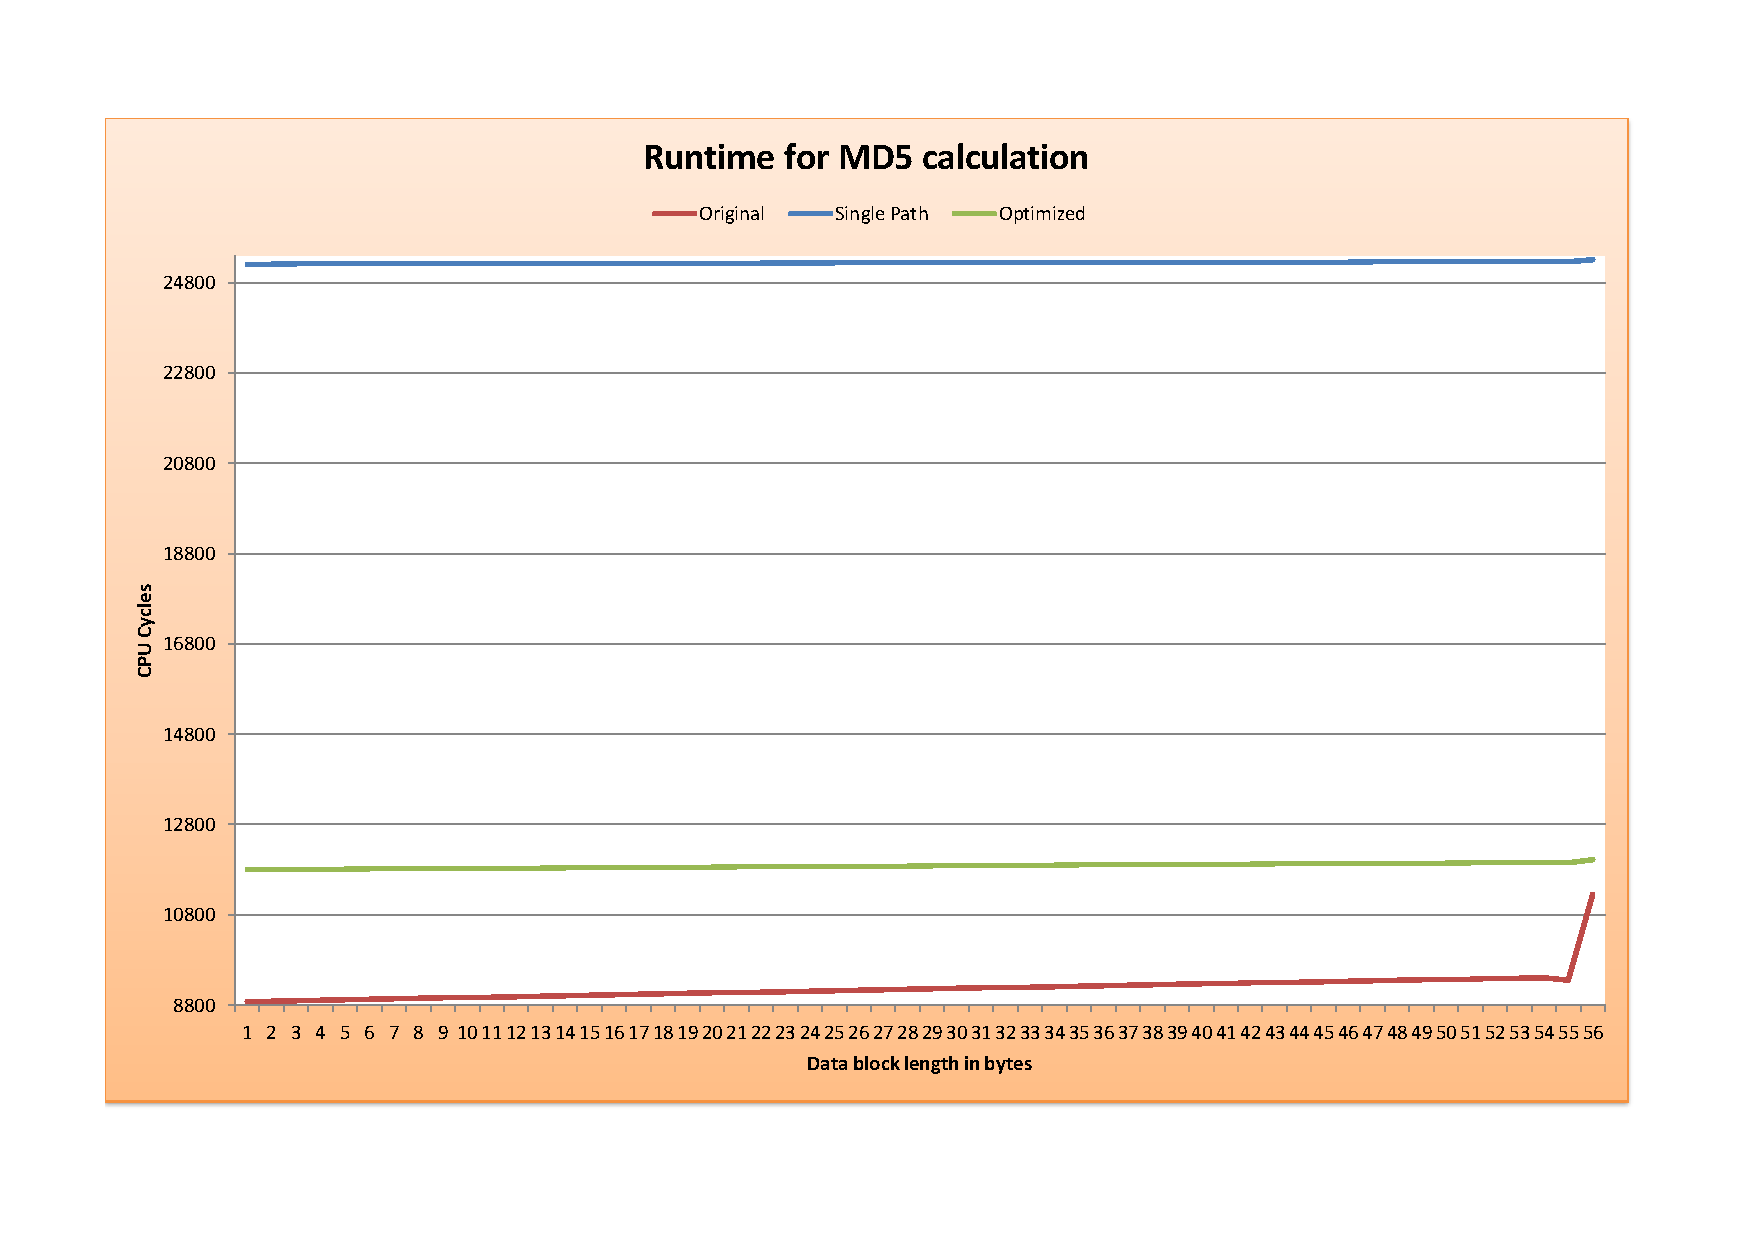
\includegraphics[height=\textwidth]{comparison.pdf}
\caption{Comparison between the three versions of the program}
\label{fig:comp}
\end{figure}
\end{landscape}

\begin{longtable}{|l|l|l|l|}
\caption{Raw measurements for big test}
\tabularnewline
\hline
\textbf{Length} & \textbf{Original} & \textbf{Single Path} & \textbf{Optimized} \tabularnewline\endhead
1&8875&25219&11799\\
2&8887&25219&11799\\
3&8895&25223&11807\\
4&8907&25223&11811\\
5&8915&25223&11811\\
6&8923&25227&11815\\
7&8935&25223&11819\\
8&8947&25227&11819\\
9&8955&25227&11823\\
10&8963&25231&11827\\
11&8975&25227&11827\\
12&8987&25231&11831\\
13&8995&25231&11835\\
14&9007&25231&11839\\
15&9015&25231&11839\\
16&9027&25235&11847\\
17&9039&25235&11847\\
18&9043&25235&11851\\
19&9059&25239&11851\\
20&9067&25239&11855\\
21&9079&25239&11859\\
22&9087&25239&11863\\
23&9095&25243&11863\\
24&9107&25239&11871\\
25&9119&25247&11871\\
26&9127&25247&11871\\
27&9135&25243&11879\\
28&9147&25243&11879\\
29&9155&25247&11883\\
30&9167&25247&11887\\
31&9179&25251&11891\\
32&9183&25247&11895\\
33&9195&25251&11895\\
34&9207&25255&11895\\
35&9215&25255&11903\\
36&9227&25251&11903\\
37&9235&25255&11907\\
38&9247&25255&11911\\
39&9259&25255&11915\\
40&9267&25259&11915\\
41&9275&25259&11919\\
42&9287&25259&11919\\
43&9295&25263&11927\\
44&9303&25263&11927\\
45&9315&25263&11931\\
46&9327&25263&11935\\
47&9339&25267&11939\\
48&9343&25267&11939\\
49&9359&25267&11943\\
50&9367&25271&11943\\
51&9375&25271&11947\\
52&9387&25271&11951\\
53&9395&25271&11955\\
54&9403&25275&11959\\
55&9351&25267&11955\\
56&11255&25311&12023\\
\hline
\textbf{Difference Max-Min}&2380&92&224\\
\hline 
\end{longtable} 

\end{document}
